\begin{table*}[t]
	\centering
	\scalebox{0.7}{
		\begin{tabular}{cc|cccccccccc|cc}
			\toprule
			Src. & Trgt. & D-MTAE~\cite{Ghifary2015mtae} & DSN~\cite{bousmalis2016domain} & CrossGrad~\cite{shankar2018generalizing} & DICA~\cite{muandet2013domaingeneralization}   &  DANN~\cite{ganin2016dann} & TF-CNN~\cite{Li2017dg}  & MetaReg~\cite{NIPS2018_metareg} & MLDG~\cite{Li2018MLDG} &  Epi-FCR~\cite{li2019episodic} & JiGen~\cite{carlucci2019domain} & Deep-All & FDM \\
			\midrule
			C,P,S&A& 60.3& 61.1 & 61.0 & 64.6& 63.2 & 62.9& 63.5 & 66.2 & 64.7 & \textbf{67.6} & 60.4 & 61.7 \\
			A,P,S&C& 58.7& 66.5 & 67.2 & 64.5 & 67.5 & 67.0&  69.5 & 66.9& 72.3 & 71.7 & 70.2 & \textbf{73.1}\\
			A,C,S&P& 91.1 & 83.3 & 87.6 & \textbf{91.8} & 88.1& 89.5&  87.4 & 88.0 & 86.1 & 89.0 & 85.3 & 87.4 \\
			A,C,P&S& 47.9& 58.6 & 55.9 & 51.1 & 57.0 & 57.5& 59.1 & 59.0 & 65.0 & \textbf{65.2} & 61.6 & 62.3 \\
			\midrule
			\multicolumn{2}{c|}{Ave.}& 64.5 &67.4 &  67.9 & 68.0& 69.0& 69.2& 69.9 & 70.0 & 72.0 & \textbf{73.4} & 69.4 & 71.1\\
			\bottomrule
	\end{tabular}}
	\vspace{-0.3cm}
	\caption{\small Cross-domain object classification results (accuracy. \%) on PACS using AlexNet.}
	\vspace{-0.4cm}
	% \vspace{-0.4cm}
	\label{tab:pacs}
\end{table*}

To demonstrate the effectiveness of the proposed method, we conduct an experiment on PACS dataset~\cite{Li2017dg} using AlexNet~\cite{Krizhevsky2012}. We follow the experiment protocol of Li~\etal~\cite{Li2017dg}. We use a batch size 512, and $\lambda$ is set to 0.1 for all tests. The results are shown in Table~\ref{tab:pacs}. As we can see, the Deep-All works better than many previous works, as Li~\etal~\cite{li2019episodic} mentioned before.

Nevertheless, the proposed method improves the performance of the Deep-All baseline. Furthermore, the proposed method shows better performance than the methods using MMD contraints~\cite{Ghifary2015mtae, muandet2013domaingeneralization}. However, the improvement is quite marginal and sub-optimal compared to state-of-the-art, which indicates the proposed regularization is quite strong.

\vspace{0.4cm}

\begin{figure}[t]
	\centering
	\footnotesize
	\begin{tabular}{c}
		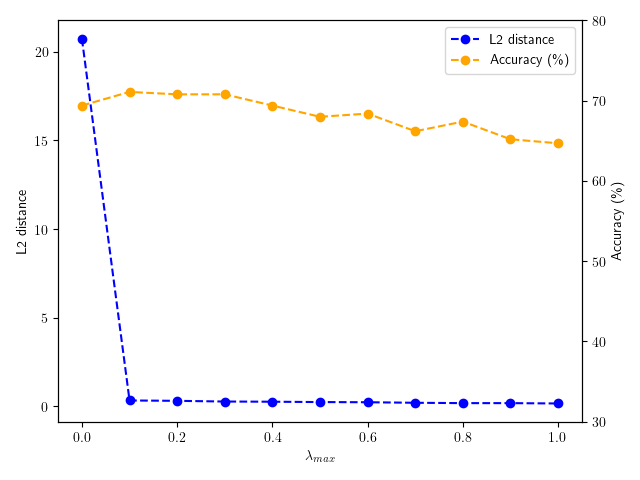
\includegraphics[width=8cm]{figures/analysis.png}
	\end{tabular}
	\caption{Analysis}\label{fig:analysis}
\end{figure}

\begin{table*}[t]
	\centering
	\scalebox{0.7}{
		\begin{tabular}{cc|cccccccc|ccc}
			\toprule
			Src. & Trgt. & D-MTAE~\cite{Ghifary2015mtae} & LRE-SVM~\cite{lresvm} & CrossGrad~\cite{shankar2018generalizing} & DICA~\cite{muandet2013domaingeneralization}   &  DANN~\cite{ganin2016dann} & MetaReg~\cite{NIPS2018_metareg} & MLDG~\cite{Li2018MLDG} &  Epi-FCR~\cite{li2019episodic} & Deep-All (\cite{li2019episodic}) & Deep-All & FDM \\
			\midrule
			L,C,S&V& 63.9& 60.6 & 65.5 & 63.7& 66.4 & 65.0 & 67.7 & 67.1 & 65.4 & 59.7 & 59.3 \\
			V,C,S&L& 60.1& 59.7 & 60.0 & 58.2 & 64.0 & 60.2 & 61.3& 64.3 & 60.6 & 54.1 & 54.3\\
			V,L,S&C& 89.1 & 88.1 & 92.0 & 79.7 & 92.6&  92.3 & 94.4 & 94.1 & 93.1 & 87.7 & 88.0 \\
			V,L,C&S& 61.3& 54.9 & 64.7 & 61.0 & 63.6 & 64.2 & 65.9 & 65.9 & 65.8 & 61.4 & 64.0 \\
			\midrule
			\multicolumn{2}{c|}{Ave.}& 68.6 &65.8 &  70.5 & 65.7 & 71.7& 70.4 & 72.3 & 72.9 & 71.2 & 65.7 & 66.4\\
			\bottomrule
	\end{tabular}}
	\vspace{-0.3cm}
	\caption{\small Cross-domain object classification results (accuracy. \%) on VLCS using AlexNet.}
	\vspace{-0.4cm}
	% \vspace{-0.4cm}
	\label{tab:vlcs}
\end{table*}

\begin{table*}[t]
	\centering
	\scalebox{0.7}{
		\begin{tabular}{cc|ccccc|ccc}
			\toprule
			Src. & Trgt. & CrossGrad~\cite{shankar2018generalizing}&  DANN~\cite{ganin2016dann} & MetaReg~\cite{NIPS2018_metareg} & MLDG~\cite{Li2018MLDG} &  Epi-FCR~\cite{li2019episodic} & Deep-All & FDM \\
			\midrule
			P,C,S&A&  78.7 & 81.3 & 79.5& 79.5 & 82.1 &  77.3 & 77.7 \\
			P,A,S&C& 73.3 & 73.8 & 75.4&  77.3 & 77.0& 73.8 & 74.2\\
			A,C,S&P& 94.0 & 94.0& 94.3&  94.3 & 93.9 & 94.1 & 94.3 \\
			P,A,C&S& 65.1 & 74.3 & 72.2& 71.5 & 73.0 & 70.8 & 71.7 \\
			\midrule
			\multicolumn{2}{c|}{Ave.}& 77.8 & 80.8 & 80.4& 80.7& 81.5  & 79.0 & 79.5 \\
			\bottomrule
	\end{tabular}}
	\vspace{-0.3cm}
	\caption{\small Cross-domain object classification results (accuracy. \%) on PACS using ResNet-18.}
	\vspace{-0.4cm}
	% \vspace{-0.4cm}
	\label{tab:pacs_resnet}
\end{table*}